%!TEX root = ClementiCooperBarba2018.tex

%* what is known
Localized surface plasmon resonance (LSPR) is an optical effect where an 
electromagnetic wave excites the free electrons on the surface of a metallic nanoparticle.
The vibrations of the electron cloud are known as plasmons, and in LSPR they resonate with the incoming
field (see Figure \ref{fig:lspr}). When this happens, most of the incoming energy
is either absorbed by the nanoparticle, or scattered in different directions,
creating a shadow behind the scatterer (a.k.a., extinction). In LSPR,
the wavelength of the incoming wave is often much larger than 
the size of the nanoparticle, 
which allows for valid approximations that simplify the mathematical model.

The phenomenon of LSPR can be used bor biosensing, 
as the resonance frequency is highly dependent on the dielectric environment 
around the scatterer. 
The resonance frequency shifts whenever an analyte binds to the nanoparticle, 
resulting in a very sensitive means of detecting its presence \cite{HaesVanduyne2002,HaesETal2004}.

Researchers using numerical models to study LSPR have mostly relied on the 
solution of Maxwell's equations in some form, using finite difference time-domain (FDTD),
boundary element, or finite element methods \cite{SolisTaboadaObelleiroLiz-MaarzanGarciadeabajo2014}. 
These simulations have been used to study the 
optical properties of dielectric or metallic nanoparticles \cite{Hohenester2018,HohenesterTrugler2012,
JungPedersenSondergaardPedersenLarsenNielsen2010, VideenSun2003,
MayergoyzFredkinZhang2005, MayergoyzZhang2007}, interactions between nanoparticles
and electron beams \cite{GarciadeabajoAizpurua1997, GarciadeabajoHowie2002},
and surface plasmon resonance sensors.
In the latter application, researchers have used simple mathematical models for the 
interaction between a metallic nanoparticle and molecules,
like representing the medium and the dissolved analytes with an effective permittivity \cite{JungCampbellChinowskyMarYee1998,HaesETal2004,PhanETal2013}. 
or representing the target molecules as spherical 
\cite{DavisGomezVernon2010,AntosiewiczApellClaudioKall2011}.

\begin{figure}[h] %  figure placement: here, top, bottom, or page
   \centering
   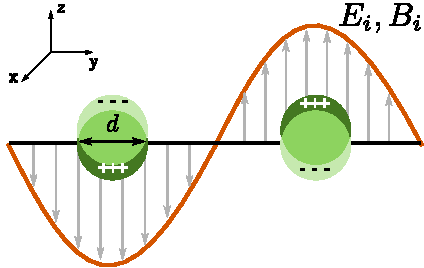
\includegraphics[width=0.35\textwidth]{lspr.pdf} 
   \caption{Illustration of the localized surface plasmon resonance (LSPR) effect of a metallic nanoparticle under an electromagnetic field. }
   \label{fig:lspr}
\end{figure}

%* What is unknown, limitations and gaps
Much of the progress in biosensor research is achieved 
through experimental investigations, often via trial and error procedures {\color{blue} I also have this impression, but do we have a reference to support it? If not, I'd rather avoid it}. 
Relying on software to assist the design process could play a key role for the manufacture 
and optimization of biosensors, giving access to details that are not available in experimental tests.
For example, empirical studies showed that the sensitivity of the sensor
is highly dependent on the distance between the nanoparticle and the analyte \cite{HaesETal2004}.
These results were modeled with a discrete dipole approximation (DDA) that does not consider the analyte in the analysis. 
Beuwer et al.~\cite{BeuwervanHoofZijlstra2018} and Henkel et al.~\cite{HenkelETal2018} used the boundary element method (BEM) to study the sensitivity of plasmonic sensors that rely on (at least) two metallic nanoparticles (one on the sensor and one attached to the analyte), also without considering the structure of the target molecule in the analysis.
While experimental evidence shows LSPR sensors are sensitive enough to detect 
conformational changes of the analytes \cite{HallETal2011}, 
current simplified models are not able to capture such details.

%* Fill the gap

Even though LSPR is an optical effect, electrostatics theory
provides a good approximation in the long-wavelength limit. This work uses
the boundary integral electrostatics solver \pygbe \cite{CooperETal2016} 
to compute the extinction cross-section of metallic nanoparticles, and to study how LSPR 
response changes in the presence of a biomolecule. 
We treat Maxwell's equations quasi-statically \cite{MayergoyzZhang2007} and
use an accurate continuum representation of the biomolecule obtained from the
crystal structure. 

\pygbe is a Python implementation of continuum electrostatic theory, used
for computing solvation energy of biomolecular systems. 
It has also been used to study protein orientation near charged nanosurfaces \cite{CooperClementiBarba2015}.
The code was recently extended to allow for complex dielectric constants 
\cite{ClementiETal2017}, aiming towards the LSPR biosensing application. 
The boundary element solver in \pygbe
is accelerated algorithmically via a treecode---an $\mathcal{O}(N\log N)$ fast solver---
and accelerated on hardware by taking advantage of
graphic processing units (GPUs). The software is shared under the BSD 3-clause license 
and is openly developed via its repository on Github.\footnote{\url{https://github.com/barbagroup/pygbe}}
This study also follows careful reproducibility practices, and all materials necessary
to reproduce the results are publicly available in reproducibility packages.
We use the Figshare and Zenodo services to deposit the computational meshes,
input and configuration files, and file bundles corresponding to the main figures in the paper.


%{\color{red}  Keeping this structure here for reference until we polish better
%the introduction.

%What is known:
%\begin{itemize}
%\item Plasmonic simulations, what applications they cover, etc. (cite Matlab guy, also Garcia de Abajo, Jung+Pedersen, etc. Maybe we can even cite COMSOL here)
%\item LSPR: how does it work, what simulations are there in the literature. Talk about work from, for example, Davis or van Duyne. See page 50 of my thesis (end chapter 2).
%\end{itemize}

%What is unkown:
%\begin{itemize}
%\item all developments are trial and error
%\item no computational tools to help in the design process
%\item example: no understanding of the sensitivity of the system
%\item models that consider the nanoparticle and the analyte are extremely simplistic
%\end{itemize}

%Fill the gap:
%\begin{itemize}
%item design of a computational tool that is highly accurate to represent the biomolecule
%\end{itemize}
%}

